\documentclass[border=8pt]{standalone}
\usepackage{tikz}
\usetikzlibrary{arrows.meta,positioning,calc}
\begin{document}
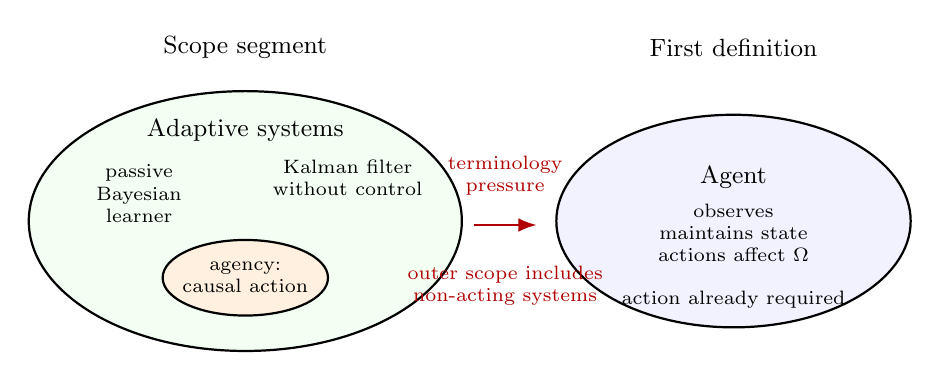
\begin{tikzpicture}[
  note/.style={align=center, font=\scriptsize},
  label/.style={align=center, font=\small},
  arr/.style={-Latex, thick}
]

% Left: broad scope from scope-adaptive-system
\node[label] at (0,2.2) {Scope segment};
\draw[thick, fill=green!5] (0,0) ellipse (2.75cm and 1.65cm);
\node[label] at (0,1.15) {Adaptive systems};
\node[note] at (-1.35,0.35) {passive\\Bayesian\\learner};
\node[note] at (1.30,0.55) {Kalman filter\\without control};
\draw[thick, fill=orange!12] (0,-0.72) ellipse (1.05cm and 0.48cm);
\node[note] at (0,-0.72) {agency:\\causal action};

% Right: first definition
\node[label] at (6.2,2.2) {First definition};
\draw[thick, fill=blue!5] (6.2,0) ellipse (2.25cm and 1.35cm);
\node[label] at (6.2,0.55) {Agent};
\node[note] at (6.2,-0.15) {observes\\maintains state\\actions affect $\Omega$};
\node[note] at (6.2,-1.0) {action already required};

\draw[arr, red!70!black] (2.9,-0.05) -- (3.7,-0.05);
\node[note, red!70!black] at (3.3,0.58) {terminology\\pressure};
\node[note, red!70!black] at (3.3,-0.82) {outer scope includes\\non-acting systems};

\end{tikzpicture}
\end{document}
